\chapter{Creating your FairShares Commons Company}
\index{FairShares Commons!company|(}
\addcontentsline{toc}{chapterdescription}{The practical chapter. You’ve decided you need your company to be at Level 5 in all three dimensions, and what to know what to do to incorporate a Level 5 FairShares Commons company. Here’s how to get your company objects / purposes, stakeholders, dilution, voting, exits, and stewardship sorted out; along with a couple of examples. See why this is the best for investors and founders, because your founding intent and values are immortalized in the principles of stewardship, and protected by the constitution through the stewards.}
\label{chapter:create-your-FSC}


\begin{chapterquotation}
In a time of destruction, create something.\\
\raggedleft\textemdash Maxine Hong Kingston\index{Kingston, Maxine Hong}
\end{chapterquotation}




The easiest way to build a FairShares Commons company\footnote{Chapter sponsored by VME Retail and Coopexchange}  is to do so when you first incorporate. 


Otherwise you hit the main roadblock to transforming an existing incorporation into a FairShares Commons: overcoming the loss-avoidance bias of existing stakeholders. 
This is not trivial, even if your most powerful stakeholders\index{stakeholders} are in agreement, because loss avoidance is one of the most powerful cognitive biases\index{biases} that humans have (Page~\pageref{section:reward-loss}). The emotion they feel at the prospect of immediate loss may well overwhelm everything that they agree with.


If you are considering a FairShares Commons incorporation, work through everything listed below with a large enough cross-section of potential stakeholders.


\begin{enumerate}
\item List out everything that your company needs to be enabled and protected at the stakeholder level. This includes the elements in your business model canvas, or whichever other approach you're using.


\item Decide which stakeholders are sufficiently central to your company’s performance so that including them in your legal incorporation will make sure it reflects what your company actually is in the lower right integral quadrant.


\item Decide the most important elements of your company's meaning\hyp{}making story. The core principles, values, and stories giving it the unique strengths that differentiate it from all others. These need to be baked into your company's statutes of incorporation, and all stewards need to exercise their vote rigorously according to these requirements. Then you have the same integrity inside your company that your conscience creates inside you.


\item Define your company's business concept. Begin by validating it through a sequence of minimum viable product types (MVP), and draft however much of your business plan is appropriate.


\item Prototype and improve the processes and structures that you need for your business from day one; and certainly long before you think of incorporating. The FairShares Commons is first and foremost an approach, an essence, not a concrete thing.
\end{enumerate}


Once you have laid out all of this, using your own tool, or the FairShares Commons business model canvas, you have the basis of what you need.


\section{Company objects, or purposes}
Strong company objects (UK), objectives (US), purposes, or whatever word is used in your country for why the company exists, build strong foundations.


Regardless of how you incorporate, without clearly defined objects you leave it open, if you are ever in a dispute, to legal people with little or even no understanding of why your company exists to make some decision what the why was at the point you created the company. In particular, they may then decide that your company only exists to provide money to financial investors.\index{investor}


Whatever purpose your company has at the point of incorporation is a consequence of whatever inner reality you were experiencing in the run-up to your decision to start up and incorporate. So as time passes, and your meaning\hyp{}making stories change, and / or actuality changes, the basis for your company's purpose may change. 


Which means that your company's purpose needs to change, if your company is to stay relevant. (Recall Chapter~\ref{section:living-organisation}.) So in a FairShares Commons, we recommend including in the statutes of incorporation the driver behind each object, or purpose\textemdash what your reality was at the time, and the need you were seeing. 


By explicitly stating the driver behind each object, it becomes very visible when the external driver has changed, and therefore the internal purpose needs to change.
\section{Stakeholder categories}
One critical concretisation of this is to lay out your initial stakeholder categories, along with how much voting weight, and share of wealth generated, is allocated to each category. A FairShares Commons company will have many or all of the following stakeholder categories.
\begin{description}
\item[Stewards] who have considerable voting power in any general meeting. They are constrained to always vote in compliance with the principles and values of stewardship as anchored in the constitution. The company’s constitution will entrench these principles and values to the same degree as the principles and values of trust are entrenched so deep that they are almost unchangeable. 


The steward category’s voting weight must be big enough that the stewards have the means to maintain the FairShares Commons integrity if any or all of the other stakeholder groups attempt, for self-interest, to treat the company in an extractive, exploitative way. The steward voting weight typically ranges from at least 26\% to 70\%, or higher if necessary.


If the steward voting weight is 100\% of the vote, then your FairShares Commons is identical to a trust or foundation in its decision process.


The stewards will meet high standards, including minimum Size of Person (Chapter~\ref{chapter:who-am-i-one}) requirements. Typically the stewards have no share of the wealth generated, but are paid a fee for their stewardship. This minimises any direct financial incentive to vote contrary to the principles that bind the steward vote (akin to how trustees are constrained legally in a trust).


Whilst a company could be a FairShares Commons in the absence of the steward class, a couple of alternatives will need to be in place. These could include a golden share, held by an actual trust, that prevents the company from being sold, or a sufficiently large number of stakeholder groups with a balance of voting weight such that it is, as near as legally allowed, impossible for the company to be sold or the constitution changed in such a way as to make the company sellable.


\item[Staff] who also have equitable voting rights in any general meeting. The staff will be accountable for representing in the general meeting the interests of current staff and, to the best extent they can, the interests of future generations of staff. They will also be expected to speak on behalf of the company and its long-term best interests from their unique perspective.


Typically the staff voting weight is equal to or slightly higher than that of any other category except steward, because the staff usually have the closest relationship with the company, living its spirit every working hour.


Staff are often more in need of immediate cash than long-term capital gain, so often they will have a higher percentage of surplus than of capital gain. For example, they may get 50\% of the surplus, but only 20\% of the capital gain.


\item[Customer, Supplier, Prosumer] representing these and analogous stakeholders. (A prosumer\index{prosumer} is the new, emerging producer-consumer. A blogger is a typical prosumer, both writing and reading blogs.) 


This may be one category, or more than one category. The important criterion in how many categories you have here is to ensure there is minimal risk of large numbers of people with one relationship to the company overwhelming a small number of people with a different relationship to the company. So, for example, if a company has a billion consumers, but only 1,000 suppliers, they ought to be in two distinct categories.


The voting weight(s), and share of surplus and appreciation, is often the smallest, as their skin in the game is least. However, if your company works with a large number of freelancers, or prosumers, you may well allocate more of the surplus and accumulation to this category than to staff or investors\index{investor}. For example, were Google \index{Google} incorporated as a FairShares Commons, \index{FairShares Commons} it might allocate the bulk of its surplus and capital gain to its individual customers.


\item[City, Nation, Environment] that the company is embedded in, perhaps even the entire planet’s natural ecosystem. In some cases, this category may have voting rights equal to or even higher than the other categories.


The share of surplus and capital gain here can be whatever is appropriate for the company’s mission and purpose. In this way, financing environmental sustainability is done directly via the company's success, on an equal footing to the financial investors' returns. The investment of natural capitals by our natural ecosystems is fully recognised within the company and its operations.


Equally, cities and nations invest infrastructure. Usually today this is paid for through taxing the company, creating a relationship of enmity between investors, and the cities or nations. So today we have suboptimal situations, where cash is extracted from companies at times when it would be actually better for everyone to leave that cash in the company. And at the other end, we have cities having to settle for a minute share of wealth generated, and directly dependent on their infrastructure investments 20 years previously. 


By cities becoming voting stakeholders they are maximally enabled to share in the company’s long-term performance, and to contribute to regenerating all kinds of built capital, getting better results in the end than they would through taxation and regulation.


I believe that this can be a very powerful way of getting an equitable split of money to all the cities and nations that are investing financial and non-financial capitals, directly and indirectly, in multinationals. The FairShares Commons incorporation eliminates much of the wrangling currently underway between nations to ensure that multinational internet companies pay a fair share towards the government-built systems their success depends on.


\item[Investor, Donor]\index{investor} are the categories for those investing or donating money in the company. These shares will be identical or close to the ordinary shares that investors are used to receiving in any company today. But the big difference, as in any FairShares company, is that these investor shares only qualify for part of the wealth generated by the company (dividends and capital gain); and, their vote is in an equitable balance to the vote of all the other stakeholders. Equitable here is based on the specific niche the company fills, and how best to bring the full breadth of relative opinions into general meeting decisions, backed by an appropriate distribution of power, for decisions to be taken in the long-term interest of the company and all of its stakeholders. 


Since all the stakeholders acquire investor shares over time, through the new shares issued each year that represent half the company’s appreciation, usually 50\% of the rise is allocated to investor shares. This is a fair reflection of the continuous investment of non-financial capitals, and is like an exchange rate connecting the different capitals invested in the company. If your investment of intellectual capital increases the company valuation, you get a fair share of that increase. Whenever you invest it, not only as a founder when the first shares are issued. 


Only the investor shares can be bought or sold. All the other share classes are cancelled without any payment as soon as the shareholder ceases to fulfil the qualification to have a share of that category. So they cannot be sold, nor be given to anyone else, nor be inherited through an estate or insolvency of a corporation holding the shares. 


Typically the only qualifying criterion to buy and hold investor shares is having money to invest, although some companies may have additional qualifying criteria. I believe that that is seldom necessary, because everything else in the FairShares Commons company means that even the greediest investor owning all the investor shares has too little power to significantly harm the interests of other stakeholders.


This is one of the big benefits of the FairShares Commons in creating regenerative businesses: the valuable power of money can be harnessed regardless of the values of the individual or corporation investing that money.


\end{description}


All the share classes can qualify for some form of sharing surplus cash, whether in the form of dividends, bonuses, or whatever is most appropriate for the company's nature and your jurisdiction. However, usually the steward share class is disqualified from receiving any wealth share in order to minimise as far as possible any conflict of interest.


Much of the wealth\index{wealth} received by all the share classes is distributed in the form of investor shares. 


For example, let's say you start working for Evolutesix,\index{Evolutesix} a FairShares Commons company. You will receive a staff share as soon as you reach the qualifying criteria, which at the moment includes working at least half of a full-time equivalent for at least six months continuously. Then, at the next wealth sharing point, you will receive investor shares according to the Evolutesix formula. This formula includes an assessment of how much the wealth generated is due to your investment, as a staff member, of different kinds of human capitals. These investor shares are now yours to sell whenever you want to. You could sell them immediately, and put cash in your pocket; or you could keep them long after you have left the company and lost your staff share, selling them in your retirement to fund your lifestyle.


As we described in the first chapters of this book, we can only build the antifragile, regenerative economy that we need if each business is an adaptive one. So make every business that you think of starting adaptive by incorporating it as a FairShares Commons, using at least self-governing structures and processes, and developmental interactions at the human level.


You can read more about how to build adaptive businesses and regenerative ecosystems of adaptive businesses in Chapter~\ref{chapter:growing-regenerative-organisations}.


I cannot stress enough the importance of all\hyp{}stakeholder dialogue. The very best way is to bring equal numbers of members of each stakeholder category into dialogue with each other, so that you can fully understand which capitals each stakeholder invests, what value / return on capitals invested each seeks, and the risks each perceives. Once you have this, then you can design the FairShares Commons company as a tool to do the job of multiplying each capital in balance with the risks to each capital. 


% DELETE?
For example, in a creator company, the creators invest significantly their risk capitals of  time, intellectual, effort, and reputation; active consumers (those who are providing active feedback,  commissioning work) are also investing the same risk capitals.
\section{Dilution, additional equity rounds}
One core element of a FairShares company is the regular issue of new investor shares to other stakeholders. Existing investors do not have an automatic right to subscribe to these new equity events, which looks like dilution through the conventional company lens. It is not dilution in the traditional context.


Dilution can be in governance power (voting) or financial wealth. 


In a FairShares Commons these share issues have no effect on\index{investor} investors’ governance power, because your voting is in specific weighted blocks; and because it is one person one vote. 


Fear of dilution on the financial side is a red herring, a cognitive bias, holding business back from thriving and generating wealth. This fear drives small-pie possessive mindsets and behaviours, when we need big-pie, commons mindsets. 


Think of having a 100g slice of a pie. Regardless of how big the pie is, your 100g slice always nourishes you with 100g of pie. If it is a 1kg pie ten people can be fed, each getting 10\% of the pie; if it is a 10kg pie 100 people can be fed, each getting 1\%. 


That is why, in the FairShares Commons, issuing new shares drives the opposite of dilution. It is exactly what enables even better success, and the biggest absolute amount of pie for you. In all capitals, not just financial. 


Worry about dilution, and you will keep the businesses you invest in smaller and weaker, on average, than they could be; and certainly far from regenerative. Focus instead on the absolute size of slice that you have, then you will work on making the business bigger and stronger for all. Which, paradoxically, means you will end up with more wealth overall; and an antifragile wealth, regardless of what percentage it is. 
\section{One person, multiple categories}
Any individual may well satisfy the qualifying criteria for multiple categories, and therefore have shares in multiple categories.


For example, the founder of a company is often in all categories. They have invested money, so have investor shares. They clearly work in the company, often with longer hours and a greater contribution to growing the business than any other member of staff, and so have staff shares; they will often also use the company’s products, and so have customer shares. Typically the founder is also a steward, because they are the source of the company, with the intuition of who the company ought to grow into.


All the other stakeholders,\index{stakeholders} after the first year at the latest, will also have investor shares. 


So, for example, staff end up with the same benefits as in an employee-owned company, and staff joining a startup later in the company's growth still benefit from equity, not just those who were in at the beginning. This also applies to any other stakeholder contributing any other capital. They all benefit from the annual cash surplus and any appreciation in company value in proportion to whatever capitals they have contributed to generating that surplus and appreciation.


Keep in mind that none of this is wildly radical, nor completely new. This is simply taking existing things, like airline miles and loyalty points, to the logical conclusion.


The stakeholders are in a rank ordering, and voting is only in the highest-ranked category that you are a member of. So anyone who is a steward and also in any of the other categories is only allowed to vote as a steward, which means that their vote is constrained to always support the principles of stewardship laid down in the constitution, and never in their own interest. The more mature the company is, the more likely that at least half of the stewards have no other significant relationship with the company.


When somebody changes their relationship with the company, and loses all other shares, they retain their investor\index{investor} shares and can still vote in the investor category. In some FairShares companies, the contribution not yet rewarded in the form of surplus or investor shares can be issued as investor shares at the point that the other shares are cancelled.


\section{Buying and selling shares}
Only the investor shares\index{investor} may be bought or sold. Depending on the details of incorporation, and company size, there will be multiple routes for investors to sell their shares. For smaller companies, that means selling the shares back to the company, or identifying another investor to buy them. For larger companies, there will be routes to sell the shares on one of the many closed markets for unlisted companies. Eventually, the publicly listed FairShares Commons company will be the dominant company on the world's largest stock markets, with a healthy trade in investor shares.


Shares of all other categories are absolutely not sellable. They are immediately withdrawn, with zero compensation, immediately any individual member ceases to fulfil the qualifying criteria.






\section{Seamless contribution and reward}
If you have a formal staff contract with any well-run company, and your work grows the business, you will receive a fair share of the wealth generated. You might get a sales commission, an annual performance bonus, stock options, a pay rise, or a promotion.


What if you are a customer, or a supplier, or the city that the company operates in, and you contribute something that grows the company’s value? In the traditional company, unless it is extraordinarily visionary, you are unlikely to get anything unless you negotiate some kind of ‘sales’ contract beforehand.


So many customers who could contribute something to a company’s success, or suppliers who could work in a seamless collaboration with the staff and perhaps customers, keep their ideas to themselves. They would rather not say anything to protect against feeling exploited if their idea generates significant wealth and they get none.


In the FairShares Commons, no matter what your relationship with the company, you are as motivated as any member of staff or investor to contribute everything you possibly can to the company’s success, because you directly get an appropriate reward. You get rewarded with a share of the surplus profit, a share of the appreciation of the company value, and a share of any of the other capitals that grow as a consequence. 


Even investors\index{investor} are more motivated to contribute and collaborate with other stakeholders to increase the company’s viability because they get more than just financial returns.


All stakeholders, \index{stakeholders} including staff, have a second motivation to contribute anything they can to the company’s success, without worrying about any contract. 


In a standard company, if a member of staff, or other stakeholders, has a really bright idea that might lead to an entirely new and profitable business unit, they may well elect to start up their own company. They do this because they have no control over what might happen to their idea in the coming decades if they simply give it to the company. It might be something with both huge profit, but also potential for environmental and social harm. So you certainly don't want to simply hand it over into a company where only investors have governance.


In the FairShares Commons, \index{FairShares Commons} members of staff and other stakeholders are far more likely to contribute everything they can to the company’s success, because they know that they have an equitable balance of governance power in the general meetings, and that the company cannot be sold to realise short-term returns for the investors only.
\section{Stewardship principles}
Getting the right stewardship principles into the company statutes and the right balance of voting power between each member categories is vital. Get this wrong, and you will not be able to use existing company law to protect the FairShares Commons characteristic of your company. Of course, the time will come when this becomes less necessary because countries will adapt their company law to include the FairShares Commons as one of their standards. Malta has already taken a significant step in this direction, by including the vanilla FairShares in its company law.


There are two types of stewardship principles in any FairShares Commons.
\begin{itemize}
\item General principles that underpin the entire FairShares Commons nature, and that must be adopted by any company wishing to be a FairShares Commons.
\item Specific principles, unique to your company, that protect and enable the core character of your company.
\end{itemize}


\subsection{General principles}
The following general principles are a minimum for a company to be deemed a FairShares Commons company.\index{FairShares Commons}
\begin{itemize}
\item To protect the company’s capacity to be a commons for its members.
\item To protect the interests of future generations, at least seven generations.
\item To protect the company’s freedom such that it cannot be bought or sold.
\item To protect against narrow interest or stakeholder groups or stakeholders gaining controlling power over the company, or the company IP curated as a commons, or the company operations, or the wealth generated by the company.
\item To foster the wise use of company IP, effort, and wealth for the good of members, human society, and natural ecosystems.
\item To foster the generation of long-term sustainable wealth across multiple capitals, including financial, human and environmental in accord with the company values.
\item To protect the FairShares principles of wealth generated being shared across members and a fair share of the right to engage in governance across those affected by governance decisions.
\item To foster the use of processes designed to surface multiple perspectives in all decisions and integrate them into a final proposal that takes into account all perspectives from all stakeholder groups, regardless of size. For example the consent / integrative decision process of sociocracy / Holacracy.
\item To protect the three Adaptive Way rules: care for self, care for the other, care for the whole. 
\end{itemize}


Also consider recording the driver (context and need) that led to this principle being part of the statutes. If the driver that led to the company being formed in the first place changes, (in other words the context and need that called the company into existence changes), you may need to also adjust any principles that were specific in their formulation to the original context and need. It is easy to see when a principle needs to be changed if the original driver is clearly articulated, because then the change in driver is visible to all.


A big driver of the growing gap in wealth in Western society is that between executive pay and the rest of the staff, let alone other stakeholders. In a FairShares Commons there is a often a maximum gap between the lowest-paid full-time employee and the highest-paid full-time employee, typically ranging from 3 to 20. 15 emerges in many polls conducted by the \emph{Economy for the Common Good}\cite{ecg-website} as the average fair point for the gap between a junior employee and senior executive pay in a large multinational. Maintaining this fairness is another role for the stewards, especially in the complex situations of a global operation that spans a wide range of local cost structures.


\section{Wealth sharing in a FairShares Commons}
Wealth, i.e. access to capital, can be shared in a FairShares Commons with every member of a company, regardless of stakeholder category, and can include all of its different capitals.


One element of this is a fair share of the financial surplus that’s generated.


Every year, in any healthy company, revenue exceeds total operating costs. After putting aside money into a pot to cover unexpected expenses in the coming years, certain types of investment, share buy-back, and other activities, the company executors may then decide to distribute any surplus to the stakeholders.


This surplus recognises the risk investment by other stakeholders of non\hyp{}financial capitals. For example, a member of staff may invest a significant number of hours without extra pay; or in the company’s early years, without any pay whatsoever. These extra hours contribute to the generation of cash flow and, somewhat akin to a performance bonus, qualify that member of staff for a fair share of the surplus. The same could apply to a member of staff who invents something, or leverages their relationships, or in any other way contributes a capital. And it applies equally well to members of any other category except investor and steward.


So any surplus is not only allocated to dividends to the investor shareholders, but is distributed in a fair way across all stakeholders to effectively reward them for their investments of non-financial risk capitals.


Profitable companies also grow in financial value. This is typically reflected in an equal growth in the price of investor shares.


In a FairShares Commons\index{FairShares Commons}, other stakeholders also benefit from that appreciation of company value. However, as no other share classes actually carry financial value, they need to be granted investor shares in proportion to how their investment of non-financial capital has helped to increase the company’s financial value.


For example, someone may join the company and bring with them an idea that leads to a new product line and a doubling of the company value. In a traditional incorporation, that person would not talk about their idea until after some return had been locked into their contract. So they might not even mention it; they might accept the job, check out the company for idea safety, and at the same time start up their own company with that idea.


In the FairShares Commons it is safe for somebody to join the company, give their idea to the company immediately without any long negotiation, and know that if the idea generates value then they will get a fair share of both the cash surplus and the appreciation of the company. This keeps a FairShares Commons in perpetual startup mode, never ossifying into a dinosaur heading to extinction because it cannot transform.


As already mentioned, the investor category\index{investor} usually gets at least 50\% of the appreciation of value. This is not only to give an adequate return on investment to the financial investors, but it also recognises that over time the contribution of other kinds of capitals underpins the continuing rise in the company’s financial value.


So in a FairShares company, if the company value doubles, instead of the investors' share price rising by 100\%, it increases by a smaller percentage, say 50\%, and the balance of the appreciation will be reflected by new shares that are distributed to the non-financial stakeholders in some proportion to their investment of non-financial capitals.
This means that all stakeholders are increasingly incentivised to collaborate in the interests of the company as a whole, because no matter what their initial capital basis was when they started engaging with the company, as time progresses they become engaged with it across all capitals.


In any FairShares company, the financial wealth generated is distributed in an equitable way across all the stakeholders investing all or any kind of capital. Even better, in a fully regenerative company that multiplies all capitals, the investors of financial capital also get a return of the wealth generated in the other capitals.


\subsection{New tax laws}
We do, however, need new tax laws. Investors of financial capital have tax breaks for gains on their investments, but the investors of human capitals and natural capitals do not yet enjoy the same benefits. This is counterproductive because the tax implications can be an insurmountable barrier for companies wishing to become the regenerative, all capitals, all stakeholders Level 5 FairShares Commons we need to create an antifragile regenerative, or even just a circular, economy. 


These tax laws also prevent the commons from working effectively as a multi-capital commons, because investments of human capital are then disadvantageously taxed to investments of financial capital, pushing us closer to civilisation collapse. 






\section{Governance is a process}
\index{consent decision making} \index{governance, FairShares}
Governance is what we call any process that carries the multiple needs, perspectives, opinions etc. within an organisation to an actionable decision. You begin developing governance processes from the very first meeting with potential co-founders when you decide to take the first step towards co-founding. So do not concretize anything into an incorporated legal framework until you know what governance process between whom (stakeholder categories) you need it to freeze and give substance to as a legal being.


Once you do incorporate as a FairShares Commons, the General Meeting is the forum for governance between stakeholder classes. Typical companies do this by simplistic voting. In a FairShares Commons, voting is the last resort and only occurs if the consent decision-making process has broken down.


A consent (not consensus) process ought to be the first option, always. It starts with one or more stakeholders recognising a new driver, or a change in an existing driver. This typically first becomes visible when they experience a conflict or tension, and use that as data on some gap, for example, between how the company is or works, and how the company ought to be or work to achieve its objects. 


After one person or a small team has clarified the tension sufficiently, and come up with a proposal for what to change to remove that tension or meet the need of the driver within the constraints of the context, this can become a topic in the general meeting. There may also be standing topics or proposals in the general meeting, such as approving the accounts for the year, executive pay, etc.


The essence of the consent decision-making process is consent to the proposal, not necessarily agreement with it. In other words, everyone can at least live with the proposal, even if they don't agree with it, or regard it as the best possible proposal. This is often expressed in the question \emph{is this good enough for now, and safe enough to try?}


There are three ways of voting in consent-based voting. 


\begin{enumerate}
\item You agree with the proposal, 
\item you disagree but can live with the proposal (consent), 
\item or you object to the proposal because you have a reason why it is not even good enough for now, and not safe enough to try once.
\end{enumerate}


If there are any objections, then every attempt is made to integrate them into a modification of the proposal. After they have been integrated, you get a new proposal, which then is put to another consent process.


The consent-based decision-making process has a number of benefits for fast-moving, adaptive businesses.


\begin{itemize}
\item Speed. Consent-based decision-making is really fast, because no one spends time trying to improve the decision beyond what is safe for now. Everyone knows that if you learn something by trying it, you can very quickly and easily run the process again to improve the decision.


\item Full data. Anyone can object, regardless of which stakeholder group they are in, or how much formal power they hold in the organisation, as long as they have a valid reason why the proposal may put the entire company at risk if it is even tried once. So proposals are only passed after all these potential reasons why have been surfaced and examined.


\item Iterative. As the consequences of any proposal become visible, the proposal can easily be revisited. This makes it easy to move fast by taking multiple safe iterative steps, rather than one risky big leap.


\item Delegated trust. Because the process surfaces a wide range of data, and there is no risk of a majority overpowering a minority, even if the minority has rightly identified a reason why the proposal is fundamentally unsafe to try even once, there is no need for everybody to attend the general meeting. If you are sufficiently confident that there is somebody else like you in the general meeting, who would surface the same objection that you might surface, you do not need to engage in the meeting. You can easily discuss your objection with that person, knowing that they will represent your perspective and without any need for you to give them a proxy vote. Also, if you look at the proposal and see that it is something you don't have a strong opinion on either way without more data, you can simply consent knowing that after it has been tried once and data is gathered, it’s easy to retake the decision.
\end{itemize}


With the advent of modern online technology to facilitate general meetings, it is easy to run a micro general meeting whenever necessary, possibly even daily!


But sometimes, the consent decision making process breaks down; for example, perhaps you can’t integrate the objections. In this case, the standard FairShares Commons weighted voting process kicks in. I recommend that a weighted vote does not happen at the same general meeting in which the consent-based decision process has broken down, especially if certain members are not present who would have been there if they’d known it would lead to a weighted vote.


In a weighted vote, the agree and consent votes are then deemed to be for the proposal, and the objections are against the proposal. Alternatively, you may in your statutes build in that only binary voting, for or against, is to be used.


Part of the stewards’ core role in the company’s early days is to articulate the values and nurture a culture that brings to life the meaning\hyp{}making essence of the company. So I recommend that their initial voting weight is high, and then steadily decreases as the company achieves specific maturity milestones. These can include the company reaching a certain age, the number of members of any category, how much has been invested, or any other appropriate indicator of members seeing it as a living being independent of themselves, and to act wisely, in loco parentis on the company’s behalf.


As mentioned before, an individual's vote only counts in the highest stakeholder category of which they are a member. This eradicates double counting.


The big benefit of this kind of voting over the traditional company structures of one share one vote, or cooperative one person one vote, is that it eliminates both kinds of tyrannies. In a typical company limited by share, the opinion that has the most money (i.e. the most voting shares) behind it wins the vote, regardless of the consequences for any other stakeholder. In the typical cooperative, the opinion with the most members behind it wins the vote, regardless of the consequences for any other stakeholder or member. 
\section{Non-profit FairShares Commons companies}
The FairShares Commons is also well-suited to the non-profit and NGO sectors. By including the full range of stakeholders in overall governance, their needs and concerns are fully represented. By being a commons, where all stakeholders are explicitly taking care of the organisation for the long term, any concerns of donors about mismanagement and misuse of funds, for example, can be effectively addressed.


For instance, Oxfam’s 2018 sex scandal has been described as a governance\cite{khan-oxfam-governance} failure. As a large global NGO, Oxfam\index{Oxfam} has needed to adopt many of the structures and practices of large for-profit multinationals. There have been criticisms of a lack of democracy, of misuse of money provided by the donor stakeholders, and of issues supporting the very stakeholders Oxfam exists to support.


Imagine if Oxfam (or choose any other NGO that you support), was structured as a non-profit FairShares Commons. Imagine how this would make it stronger, antifragile, and better enabled to do its job, because all stakeholders would be fully involved in governance. Cover-ups purely to protect one stakeholder group at the expense of others would be nearly impossible. By having all affected stakeholders directly represented in annual meetings, on the board, and in governance, all governance-related issues will be raised as soon as they begin to emerge, and used to immediately improve the NGO. The outcomes of every governance process is shaped by which stakeholders have power in the process.


Let’s stay with Oxfam\index{Oxfam} as an example. Its founders were a group of Oxford Quakers, social activists and academics. I believe that they would have immediately found their values and practices in a FairShares Commons, especially when used with the developmental and self-governing organisation components of a fully Adaptive Organisation\index{Adaptive Organisation}.
\index{FairShares Commons!companies|)}


\section{FairShares Commons canvas}
\index{FairShares Commons!canvas}
In Figure~\ref{fig:FairSharesCommons-canvas} is the canvas, derived from the lean business model canvas, we use with our clients to guide the all stakeholder dialogue needed to lay out the business model, and the enabling structures and processes needed along all three axes. 


\begin{figure}[htb]
\centering
    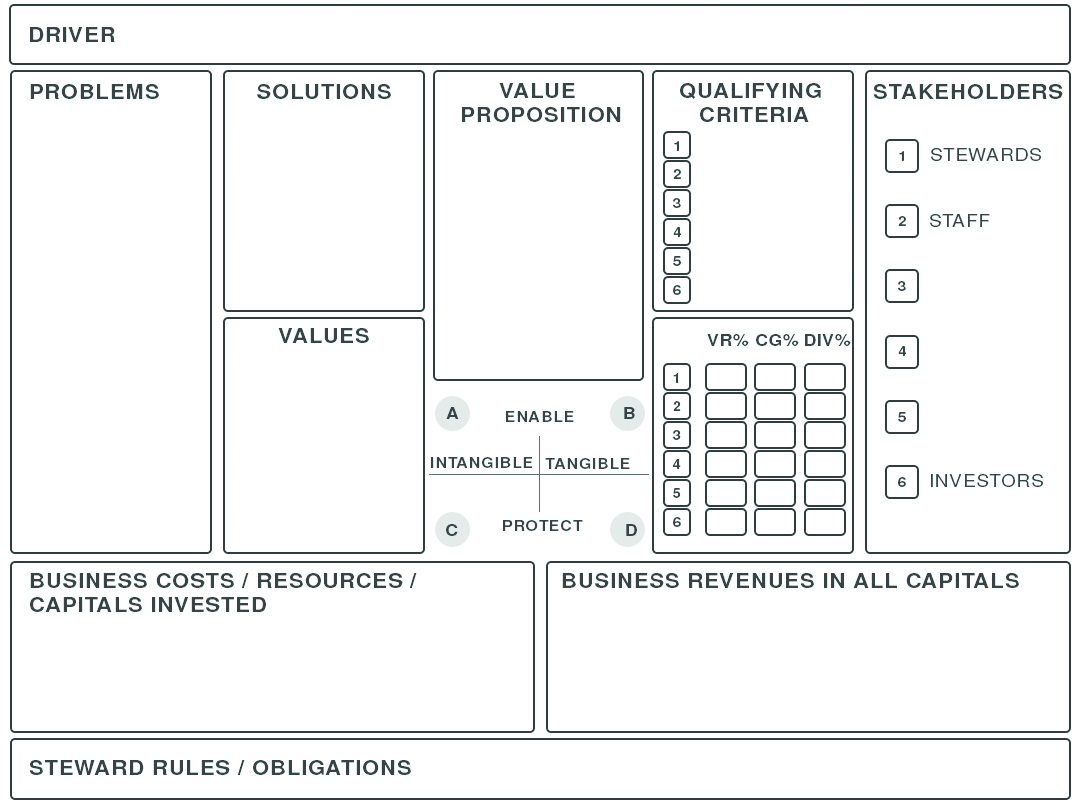
\includegraphics[
%angle=90,
width=1.00\textwidth
]{./Images/FSC-Canvas}%<---angle here
    \caption{FairShares Commons canvas.}
    \label{fig:FairSharesCommons-canvas}
\end{figure}


Fill in all the standard business elements of a lean business model canvas, or whichever conventional approach you use. Then add in all the other capitals invested in, and multiplied by the business, and the range of stakeholders investing these capitals or otherwise involved in the business. Finally, work through what the legal entity incorporation needs to enable and protect, both tangible and intangible. 


For each stakeholder, also define the minimum qualifying criteria to be eligible for membership in that stakeholder category. 


The best way to build a solid canvas is through canvassing a representative group of all stakeholders. There are many technologies for doing this, such as Open Space Technology, Appreciative Inquiry, and Future Search. There is also a wealth of useful material in the FairShares Alliance available.


And, never mistake things for processes. What matters is doing, prototyping, from day one. Long before you incorporate you ought to have identified stakeholders and begun dialogue with them, begun testing your hypotheses with them, including how governance will work between stakeholders. 
\section{Examples: UniOne and Evolutesix Publishing}
One business that I see as a superb trailblazer, and an example of how a company can be profitable (i.e., regenerative) across multiple capitals, is Whole Foods Markets, the pioneering company founded by John Mackey\index{Mackey, John}. However, when Whole Foods \index{Whole Foods Markets} began running into trouble in 2016\cite{guardian-whole-foods}, this led to activist investors buying sufficient control of the company to iteratively shift it away from conscious capitalism\index{capitalism!conscious} and towards business as usual.


If Whole Foods had been incorporated as a FairShares Commons\index{FairShares Commons}, I believe it would have had exactly the defensive power needed. The combination of governance and wealth share rights across its supplier base would have significantly increased their capacity to work with the company and make the whole ecosystem successful. The same is true for the customers, the staff, and the cities that Whole Foods is based in.


Even more, if it had been a fully Adaptive Organisation \index{Adaptive Organisation}, with all three pillars: FairShares Commons, dynamic governance, and the Adaptive Way; it would have been able to react much faster, from a higher stage of consciousness, as the competitive landscape changed around it.


Here are two companies that may one day be examples of how to build a future that works for all. 
\subsection{UniOne}
UniOne\index{UniOne|(} is an early FairShares Commons company, incorporated in 2019, with one of the authors (Graham) and Evolutesix\index{Evolutesix} playing a key role in starting it up. 


The driver for UniOne is:
\begin{quotation}
Humanity is facing a growing number of challenges of unprecedented complexity, at scales ranging from the individual through to all humanity. These challenges affect all of us, across all nations, cultures, and religions, and they span multiple disciplines. We can only address them if we work together, each of us bringing our unique strengths to bear. We also see a rise in fragmentation, from individuals who can find no peace inside their own skin, through groups, religions, organisations, nations, and between nations.


\noindent So we need better ways of enabling people to come together around what they share (oneness) and to act fully from their unique strength (uniqueness).
\end{quotation}


In order to deliver on this driver, the UniOne \index{UniOne} business model is based on a physical and a virtual platform.


Physical meetings are held, where participants are facilitated in such a way that together they can recognise and harness their common ground, whilst simultaneously each can contribute from everything that they uniquely bring. Participants learn by doing, and are then able to facilitate for others.


UniOne meetings already have a wide range, from public programs for anyone, to special interest groups for entrepreneurs, education, music, etc. It also runs training programs for people who want to develop their mastery of the UniOne methodology to become UniOne facilitators and hosts.


The virtual platform is a marketplace of prosumers, both private individuals and professionals, who offer or need a wide range of free products and services. Anyone who wants to develop themselves to their full capacity to act from the UniOne spirit in all aspects of their life needs these.


Over time, a large range of businesses and non-profit organisations will adopt the UniOne methodology, because it lets them deliver better results by leveraging everyone's common ground and thus bringing diverse unique strengths to full power. This methodology is ideally suited to any company incorporating as a FairShares Commons, and even more so to ecosystems of FairShares Commons companies.\index{FairShares Commons!companies}


The UniOne stakeholder categories, their voting weights, surplus and capital gain fractions are given in Table~\ref{table:unione-stakeholders}.
\begin{table}[htbp]
\centering  
\begin{tabular}{ c  c  c  c  c  }
\toprule
\textbf{Stakeholder} & \textbf{Initial } & \textbf{Mature }& \textbf{Appreciation }& \textbf{Surplus} \\
\textbf{} & \textbf{weight \%} & \textbf{weight \%}& \textbf{share \%}& \textbf{share \%} \\
        \midrule
 Steward & 60 & 40 & 0 & 0 \\
 Staff & 8 & 13 & 20 & 30 \\
 Individual Prosumer & 8 & 16 & 15 & 20 \\
 Professional Prosumer & 7 & 9 & 15 & 25 \\
 Donors & 7 & 7 & 0 & 0 \\
 Investors & 10 & 15 & 50 & 25 \\
\bottomrule
\end{tabular}
\caption[Stakeholder categories in UniOne]{Table of the different stakeholder categories in UniOne}
\label{table:unione-stakeholders}
\end{table}


Because UniOne is very centred on staying true to its spirit, the steward voting weight will be a high 40\% when mature. The group of stewards themselves include representatives from each other category, a member from the UniOne non-profit foundation, and external appointed members. This minimises the risk of stewards lacking the breadth, depth, and independence of perspective to wisely guide UniOne according to its spirit.


It is going to take time, with various experiments and interpretations, before the UniOne spirit and its business structures and processes can be clearly and unambiguously articulated in words. So the initial voting weight of the stewards is an even higher 60\%.


The stewards do not benefit directly from any cash surplus distributed, nor from UniOne’s capital gain. However, those founders that also have a steward role all have investor shares, representing their significant investment of time and money, which enable them to benefit from their investment. However, they have no vote in the investor class, though\textemdash keep in mind that their vote is always constrained by the principles anchored in the statutes, and they can be held legally accountable if it breaks these principles.


You also see that the donors have zero return from surplus or capital gain. In many countries, any benefit nullifies a donor’s right to tax rebates.


The remaining voting weights are distributed in such a way that the number of members in each stakeholder category balances out in an equitable way in any decision. This means that if the consent process breaks down, UniOne decisions are neither dominated by the opinion with the largest number of people, nor by the opinion with the largest amount of money.


Equally, the share of wealth is designed to reflect the needs and scale of contribution expected from each class to the success of UniOne as a whole. \index{UniOne|)}
\subsection{Evolutesix Publishing}
We are creating it in part to make ensure that the company publishing this book walks the talk; and as an example of what Evolutesix\index{Evolutesix} is doing to incubate and invest in ecosystems of FairShares Commons companies.


The driver for Evolutesix Publishing is:
\begin{quotation}
Publishing is a tool to disseminate information from where it is, to where it is needed. The publishing industry today, especially academic publishing and publishing the first books in contentious fields, or those that challenge existing paradigms, is no longer up to the task. Knowledge behaves differently to other capitals, in that if two people give each other new knowledge that the other lacks, both now have both knowledge. Knowledge multiplies when it is shared. The mutually beneficial share of value created across all stakeholders is broken in current publishing, to the detriment of the primary value creators\textemdash the authors and readers.


\noindent We need a new platform approach to publishing with a business model based on the value-add when knowledge is shared widely, disseminated rapidly, and integrated. To do this, we need a publishing business that integrates all of the emerging information technologies under a commons business model.
\end{quotation}


Evolutesix Publishing intends to publish the new paradigms in economics, regenerative business, sustainability, community, identity, etc. 


At the heart of Evolutesix Publishing is a crowd paradigm. Authors and readers will form a vibrant interacting community, where the readers support the writer during the process of writing the book and afterwards. This can be in the form of regular discussions with the author, to streamline and improve the connection between the book (content and style) and the reader.


This makes far easier things like crowdfunding, crowdsourcing, and even writing the entire book as a crowd of authors. The division between reader and author becomes far more fluid.


This also takes us beyond the book writing process of: get it right, publish it, and then leave it for a few years, until enough changes have accumulated to warrant a new edition.


This leads to the current proposal for our stakeholder split, in Table~\ref{table:publishing-stakeholders}. At the point of publishing this book Evolutesix Publishing is still in the creation phase, and has yet to be incorporated as an independent company from Evolutesix itself. So these may well change as we continue to get input during the early stages of the company.


\begin{table}[htbp]
\centering  
\begin{tabular}{ c  c  c  c  c  }
\toprule
\textbf{Stakeholder} & \textbf{Initial } & \textbf{Mature }& \textbf{Appreciation }& \textbf{Surplus} \\
\textbf{} & \textbf{weight \%} & \textbf{weight \%}& \textbf{share \%}& \textbf{share \%} \\
        \midrule
 Steward  & 70 & 30     & 0       & 0 \\
 Staff        & 10  & 20    & 20     & 25 \\
 Authors   & 5   & 12.5  & 12.5  & 20 \\
 Readers  & 5   & 12.5  & 12.5  & 20 \\
 Suppliers & 0   & 5       & 5       & 5 \\
 Investors & 10 & 20     & 50     & 30 \\
\bottomrule
\end{tabular}
\caption[Stakeholder categories in Evolutesix Publishing]{Table of the different stakeholder categories in Evolutesix Publishing}
\label{table:publishing-stakeholders}
\end{table}






\section{Transforming dominant paradigms}
\begin{quote}
And day to day, life's a hard job, you get tired, you lose the pattern. You need distance, interval.\\
\raggedleft\textemdash Ursula K. Le Guin\index{Le Guin, Ursula K.}
\end{quote}


Every one of us who is going on the journey to creating a future that we can all thrive in has chosen the hardest job there is, transforming our dominant paradigms and the institutions they have been concretised into. 


We will all get tired and want to give up at times. I know I do. What keeps me (Graham) going is remembering others who have gone on even harder journeys, and then seeing what I can learn from their journey. 


There are four lessons from what worked in transforming South Africa\index{South Africa} to re-apply to business.


\begin{enumerate}
\item Freedom is the foundation. Each company must be free, not subject to single-class ownership. Then everyone can have the psychological safety\index{psychological safety} that comes with being fully enfranchised and having full information rights. Only then is it really safe to use the full power of any of the Ocracies\cite{robertson-holacracy, rau-sociocracy}, and / or Deliberately Developmental\cite{kegan-everyone} methods.\index{Kegan, Robert}
\item Include everyone in the process, in the benefits, and in the costs, especially those you see as “the other”. Climate change \index{climate!change} has occurred because we externalise the costs onto others (especially future generations, our children and grandchildren). Once we no longer see “others”, externalising costs becomes visible as self-harm.
\item Human beings have written our company statutes, our stories of how things must work. So humans like you and me can rewrite them now.
\item Quick successes first. Use existing legal constructs and loopholes creatively to do it now, even if not perfectly. The FairShares Commons Incorporation is already being implemented in the UK, many other countries in the EU, Nigeria, and the USA.
\end{enumerate}




In closing, it is my belief that the Adaptive Organisation,\index{Adaptive Organisation} with all three axes at Level~5, may well be the new cooperativism we need, may well be the basis for Impact Investing Plus, and what we require to regenerate our planet and society, to address the climate emergency and achieve the 17 Sustainable Development Goals. \index{Sustainable Development Goals, UN 17}